\documentclass[11pt, a4paper]{article}

% Fonts and Encoding
\usepackage[utf8]{inputenc}
\usepackage[T1]{fontenc}

% Math and Symbols
\usepackage{amsmath, amssymb, amsthm, amsfonts, mathrsfs, mathtools}

% Layout and Geometry
\usepackage{geometry}
\geometry{a4paper, margin=1in}

% Formatting and Graphics
\usepackage{graphicx, xcolor, enumitem, booktabs, array, tabularx}

% TikZ for Illustrations
\usepackage{tikz}
\usetikzlibrary{arrows.meta, positioning, shapes.geometric, calc, backgrounds, matrix}

% Clickable Links and TOC
\usepackage{hyperref}
\hypersetup{
    colorlinks=true,
    linkcolor=blue,
    filecolor=magenta,      
    urlcolor=cyan,
    pdftitle={Comprehensive Guide to Laplace Transforms},
}

% Theorem Environments
\newtheorem{theorem}{Theorem}[section]
\newtheorem{lemma}[theorem]{Lemma}
\newtheorem{proposition}[theorem]{Proposition}
\newtheorem{corollary}[theorem]{Corollary}
\theoremstyle{definition}
\newtheorem{definition}{Definition}[section]
\newtheorem{axiom}{Axiom}[section]
\newtheorem{example}{Example}[section]
\theoremstyle{remark}
\newtheorem{remark}{Remark}[section]

% Custom Commands (Enforced standard notation)
\newcommand{\R}{\mathbb{R}}
\newcommand{\N}{\mathbb{N}}
\newcommand{\Z}{\mathbb{Z}}
\newcommand{\Q}{\mathbb{Q}}
\newcommand{\E}{\mathbb{E}}
\newcommand{\Prob}{\mathbb{P}}
\newcommand{\F}{\mathcal{F}}

\title{Comprehensive Guide to Laplace Transforms}
\author{Tashfeen Omran}
\date{\today}

\begin{document}

\maketitle
\tableofcontents
\newpage

\section{Comprehensive Introduction, Context, and Prerequisites}

\subsection{Core Concepts}
The Laplace Transform is a powerful integral transform used to switch a function from the time domain (usually represented by the variable $t$) to the frequency domain (represented by the complex variable $s$). In essence, it takes a differential equation, which is often difficult to solve directly, and transforms it into an algebraic equation, which is much easier to manipulate. Once the algebraic equation is solved in the $s$-domain, an Inverse Laplace Transform is applied to map the solution back to the time domain.

\subsection{Intuition and Derivation}
The Laplace Transform can be thought of as a continuous analog of a power series. While a power series $\sum a_n x^n$ encodes a discrete sequence $a_n$ into a continuous function of $x$, the Laplace Transform encodes a continuous function $f(t)$ into a new function $F(s)$. 

Mathematically, the Laplace Transform of a function $f(t)$, defined for all $t \ge 0$, is given by the improper integral:
\[
\mathscr{L}\{f(t)\} = F(s) = \int_0^\infty e^{-st} f(t) \, dt
\]
The term $e^{-st}$ acts as a damping factor. For functions $f(t)$ that do not grow faster than an exponential function (i.e., functions of exponential order), this damping factor ensures that the improper integral converges for sufficiently large values of $s$.

\begin{center}
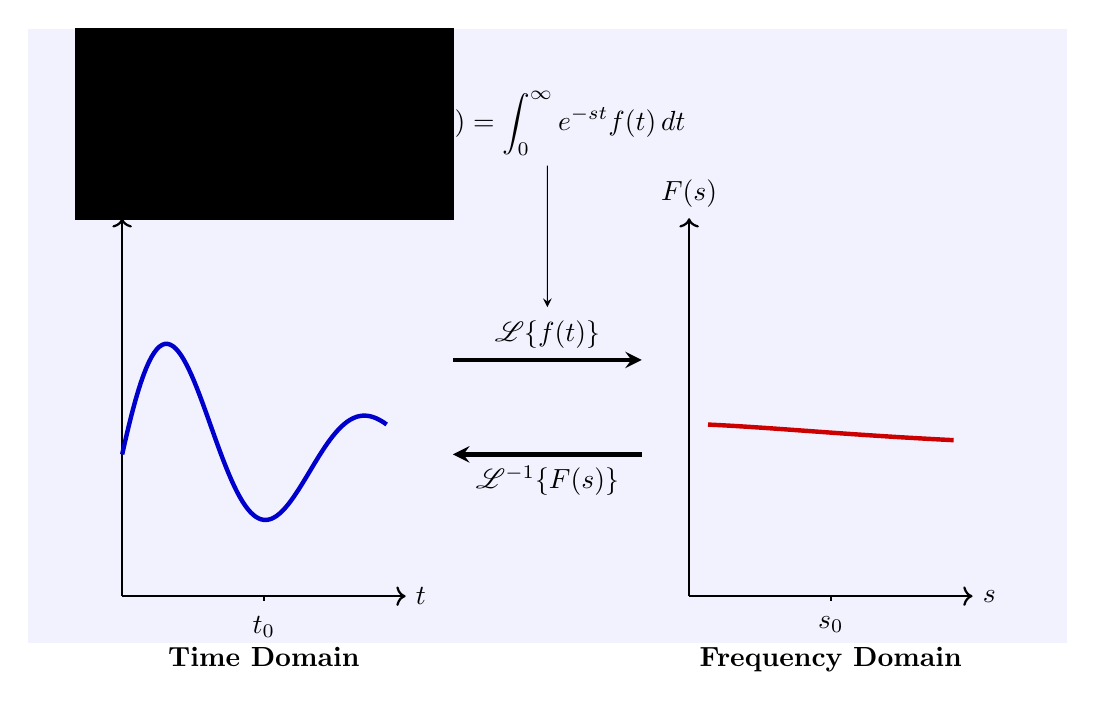
\begin{tikzpicture}[scale=1.2]
    % 1) Background
    \fill[blue!5] (-1,-2) rectangle (10, 4.5);
    
    % 2) Grid lines/axes
    \draw[thick, ->] (0,-1.5) -- (3,-1.5) node[right] {$t$};
    \draw[thick, ->] (0,-1.5) -- (0,2.5) node[above] {$f(t)$};
    \draw[thick, ->] (6,-1.5) -- (9,-1.5) node[right] {$s$};
    \draw[thick, ->] (6,-1.5) -- (6,2.5) node[above] {$F(s)$};
    
    % Microscopic tick marks
    \draw[thick] (1.5, -1.5) -- (1.5, -1.55) node[below=2pt, black] {$t_0$};
    \draw[thick] (7.5, -1.5) -- (7.5, -1.55) node[below=2pt, black] {$s_0$};
    
    % 3) Primary plots
    \draw[ultra thick, blue!80!black, domain=0:2.8, samples=100] plot (\x, {1.5*exp(-0.5*\x)*sin(deg(3*\x))});
    \draw[ultra thick, red!80!black, domain=6.2:8.8, samples=100] plot (\x, {3/(((\x-6)+0.5)^2 + 9)});
    
    % 4) Node labels/text
    \node[below=15pt, black] at (1.5,-1.5) {\textbf{Time Domain}};
    \node[below=15pt, black] at (7.5,-1.5) {\textbf{Frequency Domain}};
    
    % Transform Arrows
    \draw[ultra thick, ->, >=stealth] (3.5, 1) -- (5.5, 1) node[midway, above, black] {$\mathscr{L}\{f(t)\}$};
    \draw[ultra thick, <-, >=stealth] (3.5, 0) -- (5.5, 0) node[midway, below, black] {$\mathscr{L}^{-1}\{F(s)\}$};
    
    % Legend (Single-Node Multiline Rule, Anchor Pivot Strategy)
    \node[align=left, anchor=west, draw, fill=white, inner sep=8pt, black] at (-0.5, 3.5) {
        \textbf{Domain Transformation} \\[4pt]
        Blue: $\displaystyle f(t) = e^{-0.5t}\sin(3t)$ \\[4pt]
        Red: $\displaystyle F(s) = \frac{3}{(s+0.5)^2 + 9}$
    };
    
    % Off-Axis Callout
    \node[align=left, black] (integral) at (4.5, 3.5) {$\displaystyle F(s) = \int_0^\infty e^{-st} f(t) \, dt$};
    \draw[->, >=stealth, shorten >=2pt, thin] (integral) -- (4.5, 1.5);
\end{tikzpicture}
\end{center}

\subsection{Historical Context and Motivation}
The transform is named after the brilliant French mathematician Pierre-Simon Laplace, who introduced it in his work on probability theory in the late 18th century. However, the true operational power of the transform was popularized much later by the English electrical engineer Oliver Heaviside in the late 19th century. Heaviside developed an "operational calculus" to solve complex differential equations in electrical circuits by treating the differential operator as an algebraic variable. The Laplace Transform provided the rigorous mathematical foundation for Heaviside's highly successful, yet initially unproven, techniques.

\subsection{Key Formulas}
The following table summarizes the foundational Laplace Transforms.

\renewcommand{\arraystretch}{1.5}
\noindent
\begin{tabularx}{\textwidth}{>{$\displaystyle}c<{$} >{$\displaystyle}X<{$}}
\toprule
\text{\textbf{Function} } f(t) & \text{\textbf{Laplace Transform} } F(s) = \mathscr{L}\{f(t)\} \\
\midrule
1 & \frac{1}{s}, \quad s > 0 \\
\addlinespace[4pt]
e^{at} & \frac{1}{s-a}, \quad s > a \\
\addlinespace[4pt]
t^n & \frac{n!}{s^{n+1}}, \quad s > 0 \\
\addlinespace[4pt]
\sin(bt) & \frac{b}{s^2+b^2}, \quad s > 0 \\
\addlinespace[4pt]
\cos(bt) & \frac{s}{s^2+b^2}, \quad s > 0 \\
\addlinespace[4pt]
e^{at} f(t) & F(s-a) \quad \text{(First Translation Theorem)} \\
\addlinespace[4pt]
t^n f(t) & (-1)^n \frac{d^n}{ds^n} F(s) \quad \text{(Derivative of Transform)} \\
\bottomrule
\end{tabularx}

\subsection{Prerequisites}
To master this topic, you must be highly proficient in:
\begin{itemize}
    \item \textbf{Algebraic Expansion:} Expanding polynomials (e.g., Binomial Theorem) and completing the square.
    \item \textbf{Trigonometric Identities:} Specifically, half-angle formulas ($\sin^2 \theta$, $\cos^2 \theta$) and product-to-sum formulas.
    \item \textbf{Differentiation Rules:} The quotient rule and chain rule are heavily used when applying the derivative of a transform property.
    \item \textbf{Improper Integrals:} Understanding limits at infinity, which forms the basis of the transform's definition.
\end{itemize}

\newpage

\section{Detailed Homework Solutions}

\subsection{Problem 1}
\textbf{Evaluate:} $\mathscr{L}\{e^{-7t} \cos 4t + e^t - 1\}$

\textbf{Solution:}
By the linearity of the Laplace Transform, we can split the expression into three separate transforms:
\[
\mathscr{L}\{e^{-7t} \cos 4t\} + \mathscr{L}\{e^t\} - \mathscr{L}\{1\}
\]
For the first term, we use the standard transform for cosine and apply the First Translation Theorem (shifting property) due to the $e^{-7t}$ multiplier.
\[
\mathscr{L}\{\cos 4t\} = \frac{s}{s^2 + 16} \implies \mathscr{L}\{e^{-7t} \cos 4t\} = \frac{s+7}{(s+7)^2 + 16}
\]
For the second and third terms, we use the standard table values:
\[
\mathscr{L}\{e^t\} = \frac{1}{s-1}, \quad \mathscr{L}\{1\} = \frac{1}{s}
\]
Combining all the terms yields the final answer:
\[
\frac{s+7}{(s+7)^2 + 16} + \frac{1}{s-1} - \frac{1}{s}
\]

\subsection{Problem 2}
\textbf{Evaluate:} $\mathscr{L}\{t^2 e^{-5t} - t^3 + \cos 3t\}$

\textbf{Solution:}
Apply linearity to separate the terms:
\[
\mathscr{L}\{t^2 e^{-5t}\} - \mathscr{L}\{t^3\} + \mathscr{L}\{\cos 3t\}
\]
For the first term, we find the transform of $t^2$ and shift it by $s \to s+5$:
\[
\mathscr{L}\{t^2\} = \frac{2!}{s^3} = \frac{2}{s^3} \implies \mathscr{L}\{t^2 e^{-5t}\} = \frac{2}{(s+5)^3}
\]
For the second term, we use the power rule $\mathscr{L}\{t^n\} = \frac{n!}{s^{n+1}}$:
\[
\mathscr{L}\{t^3\} = \frac{3!}{s^4} = \frac{6}{s^4}
\]
For the third term, we use the standard cosine transform:
\[
\mathscr{L}\{\cos 3t\} = \frac{s}{s^2 + 9}
\]
Combining the results:
\[
\frac{2}{(s+5)^3} - \frac{6}{s^4} + \frac{s}{s^2 + 9}
\]

\subsection{Problem 3}
\textbf{Evaluate:} $\mathscr{L}\{(t+2)^4\}$

\textbf{Solution:}
The Laplace Transform does not distribute over powers. We must first expand the polynomial using the Binomial Theorem:
\[
(t+2)^4 = t^4 + 4t^3(2) + 6t^2(4) + 4t(8) + 16 = t^4 + 8t^3 + 24t^2 + 32t + 16
\]
Now, apply the Laplace Transform to each term individually using $\mathscr{L}\{t^n\} = \frac{n!}{s^{n+1}}$:
\[
\mathscr{L}\{t^4\} + 8\mathscr{L}\{t^3\} + 24\mathscr{L}\{t^2\} + 32\mathscr{L}\{t\} + 16\mathscr{L}\{1\}
\]
\[
= \frac{4!}{s^5} + 8\left(\frac{3!}{s^4}\right) + 24\left(\frac{2!}{s^3}\right) + 32\left(\frac{1!}{s^2}\right) + 16\left(\frac{1}{s}\right)
\]
Simplify the factorials:
\[
= \frac{24}{s^5} + \frac{48}{s^4} + \frac{48}{s^3} + \frac{32}{s^2} + \frac{16}{s}
\]

\subsection{Problem 4}
\textbf{Evaluate:} $\mathscr{L}\{(3 + e^{-2t})^2\}$

\textbf{Solution:}
Similar to the previous problem, we must expand the square first:
\[
(3 + e^{-2t})^2 = 9 + 2(3)(e^{-2t}) + (e^{-2t})^2 = 9 + 6e^{-2t} + e^{-4t}
\]
Apply the Laplace Transform to each term:
\[
\mathscr{L}\{9\} + 6\mathscr{L}\{e^{-2t}\} + \mathscr{L}\{e^{-4t}\}
\]
Using the standard transforms for constants and exponentials:
\[
= \frac{9}{s} + \frac{6}{s+2} + \frac{1}{s+4}
\]

\subsection{Problem 5}
\textbf{Evaluate:} $\mathscr{L}\{t e^t \cos t\}$

\textbf{Solution:}
This problem requires a two-step process. First, we handle the exponential shift, and then we handle the multiplication by $t$.
Step 1: Find the transform of $e^t \cos t$.
\[
\mathscr{L}\{\cos t\} = \frac{s}{s^2 + 1}
\]
By the First Translation Theorem, shifting $s \to s-1$:
\[
\mathscr{L}\{e^t \cos t\} = \frac{s-1}{(s-1)^2 + 1} = \frac{s-1}{s^2 - 2s + 2}
\]
Step 2: Apply the derivative property for multiplication by $t$. The property states $\mathscr{L}\{t f(t)\} = -\frac{d}{ds} F(s)$.
\[
\mathscr{L}\{t e^t \cos t\} = -\frac{d}{ds} \left( \frac{s-1}{s^2 - 2s + 2} \right)
\]
Apply the quotient rule:
\[
= -\frac{1 \cdot (s^2 - 2s + 2) - (s-1)(2s - 2)}{(s^2 - 2s + 2)^2}
\]
Factor out a $2$ from the second term in the numerator:
\[
= -\frac{s^2 - 2s + 2 - 2(s-1)^2}{(s^2 - 2s + 2)^2}
\]
Expand $(s-1)^2$:
\[
= -\frac{s^2 - 2s + 2 - 2(s^2 - 2s + 1)}{(s^2 - 2s + 2)^2}
\]
Simplify the numerator:
\[
= -\frac{s^2 - 2s + 2 - 2s^2 + 4s - 2}{(s^2 - 2s + 2)^2} = -\frac{-s^2 + 2s}{(s^2 - 2s + 2)^2}
\]
Final Answer:
\[
\frac{s^2 - 2s}{(s^2 - 2s + 2)^2}
\]

\subsection{Problem 6}
\textbf{Evaluate:} $\mathscr{L}\{\cosh bt\}$

\textbf{Solution:}
The hyperbolic cosine function is defined in terms of exponentials:
\[
\cosh bt = \frac{e^{bt} + e^{-bt}}{2}
\]
Apply the Laplace Transform using linearity:
\[
\mathscr{L}\{\cosh bt\} = \frac{1}{2} \mathscr{L}\{e^{bt}\} + \frac{1}{2} \mathscr{L}\{e^{-bt}\}
\]
\[
= \frac{1}{2} \left( \frac{1}{s-b} + \frac{1}{s+b} \right)
\]
Find a common denominator to combine the fractions:
\[
= \frac{1}{2} \left( \frac{(s+b) + (s-b)}{(s-b)(s+b)} \right) = \frac{1}{2} \left( \frac{2s}{s^2 - b^2} \right)
\]
Final Answer:
\[
\frac{s}{s^2 - b^2}
\]

\subsection{Problem 7}
\textbf{Evaluate:} $\mathscr{L}\{15 \sin^2 5t\}$

\textbf{Solution:}
We cannot directly transform $\sin^2 \theta$. We must use the power-reducing (half-angle) trigonometric identity: $\sin^2 \theta = \frac{1 - \cos 2\theta}{2}$.
\[
15 \sin^2 5t = 15 \left( \frac{1 - \cos 10t}{2} \right) = \frac{15}{2} - \frac{15}{2} \cos 10t
\]
Now, apply the Laplace Transform:
\[
\mathscr{L}\left\{\frac{15}{2}\right\} - \mathscr{L}\left\{\frac{15}{2} \cos 10t\right\}
\]
\[
= \frac{15}{2s} - \frac{15}{2} \left( \frac{s}{s^2 + 100} \right)
\]
Combine into a single fraction by finding a common denominator:
\[
= \frac{15(s^2 + 100) - 15s(s)}{2s(s^2 + 100)} = \frac{15s^2 + 1500 - 15s^2}{2s(s^2 + 100)}
\]
Final Answer:
\[
\frac{750}{s(s^2 + 100)}
\]

\subsection{Problem 8}
\textbf{Evaluate:} $\mathscr{L}\{\sin 5t \sin 3t\}$

\textbf{Solution:}
We must convert the product of sines into a sum using the product-to-sum trigonometric identity: $\sin A \sin B = \frac{1}{2} [\cos(A-B) - \cos(A+B)]$.
\[
\sin 5t \sin 3t = \frac{1}{2} [\cos(5t - 3t) - \cos(5t + 3t)] = \frac{1}{2} [\cos 2t - \cos 8t]
\]
Apply the Laplace Transform:
\[
\frac{1}{2} \mathscr{L}\{\cos 2t\} - \frac{1}{2} \mathscr{L}\{\cos 8t\}
\]
\[
= \frac{1}{2} \left( \frac{s}{s^2 + 4} \right) - \frac{1}{2} \left( \frac{s}{s^2 + 64} \right)
\]
Combine into a single fraction:
\[
= \frac{s(s^2 + 64) - s(s^2 + 4)}{2(s^2 + 4)(s^2 + 64)} = \frac{s^3 + 64s - s^3 - 4s}{2(s^2 + 4)(s^2 + 64)} = \frac{60s}{2(s^2 + 4)(s^2 + 64)}
\]
Final Answer:
\[
\frac{30s}{(s^2 + 4)(s^2 + 64)}
\]

\subsection{Problem 9}
\textbf{Evaluate using the formula $\mathscr{L}\{t^n f(t)\} = (-1)^n \frac{d^n}{ds^n} F(s)$:}
\textbf{(a)} $\mathscr{L}\{t \cos bt\}$
\textbf{(b)} $\mathscr{L}\{t^2 \cos bt\}$

\textbf{Solution (a):}
Here $f(t) = \cos bt$, so $F(s) = \frac{s}{s^2 + b^2}$, and $n=1$.
\[
\mathscr{L}\{t \cos bt\} = - \frac{d}{ds} \left( \frac{s}{s^2 + b^2} \right)
\]
Apply the quotient rule:
\[
= - \frac{1 \cdot (s^2 + b^2) - s(2s)}{(s^2 + b^2)^2} = - \frac{s^2 + b^2 - 2s^2}{(s^2 + b^2)^2} = - \frac{b^2 - s^2}{(s^2 + b^2)^2}
\]
Final Answer (a):
\[
\frac{s^2 - b^2}{(s^2 + b^2)^2}
\]

\textbf{Solution (b):}
Here $n=2$. We can take the derivative of the result from part (a) and multiply by $-1$, since $\mathscr{L}\{t^2 \cos bt\} = -\frac{d}{ds} \mathscr{L}\{t \cos bt\}$.
\[
\mathscr{L}\{t^2 \cos bt\} = - \frac{d}{ds} \left( \frac{s^2 - b^2}{(s^2 + b^2)^2} \right)
\]
Apply the quotient rule carefully:
\[
= - \frac{2s(s^2 + b^2)^2 - (s^2 - b^2) \cdot 2(s^2 + b^2)(2s)}{(s^2 + b^2)^4}
\]
Factor out $(s^2 + b^2)$ from the numerator to simplify:
\[
= - \frac{(s^2 + b^2) [ 2s(s^2 + b^2) - 4s(s^2 - b^2) ]}{(s^2 + b^2)^4}
\]
Cancel the common factor and expand the brackets:
\[
= - \frac{2s^3 + 2sb^2 - 4s^3 + 4sb^2}{(s^2 + b^2)^3} = - \frac{-2s^3 + 6sb^2}{(s^2 + b^2)^3}
\]
Final Answer (b):
\[
\frac{2s^3 - 6sb^2}{(s^2 + b^2)^3}
\]

\subsection{Problem 10}
\textbf{Given $\mathscr{L}\{\cos bt\} = \frac{s}{s^2 + b^2}$, use the translation property to compute $\mathscr{L}\{e^{at} \cos bt\}$.}

\textbf{Solution:}
The First Translation Theorem states that if $\mathscr{L}\{f(t)\} = F(s)$, then multiplying the time-domain function by $e^{at}$ results in a shift in the frequency domain: $\mathscr{L}\{e^{at} f(t)\} = F(s-a)$.
Given $F(s) = \frac{s}{s^2 + b^2}$, we substitute $(s-a)$ for every instance of $s$.
Final Answer:
\[
\frac{s-a}{(s-a)^2 + b^2}
\]

\newpage

\section{In-Depth Analysis of Problems and Techniques}

\subsection{Problem Types and General Approach}
The homework assignment can be categorized into four distinct problem types:
\begin{enumerate}
    \item \textbf{Direct Table Application \& Linearity (Problems 1, 2):} These problems require breaking down a sum of functions into individual components and applying standard table formulas. The general strategy is to distribute the Laplace operator and handle each term independently.
    \item \textbf{Algebraic Expansion (Problems 3, 4):} The Laplace Transform is a linear operator; it does not distribute over multiplication or powers. The strategy here is to completely expand polynomials (using the Binomial Theorem) or perfect squares before applying the transform.
    \item \textbf{Trigonometric Identities (Problems 6, 7, 8):} Transforms of squared trigonometric functions or products of trigonometric functions do not exist in standard tables. The strategy is to use power-reducing formulas or product-to-sum formulas to convert these expressions into linear combinations of sine and cosine functions with modified frequencies.
    \item \textbf{Operational Properties (Problems 5, 9, 10):} These problems test the structural properties of the transform. The strategy involves recognizing multipliers like $e^{at}$ (which triggers an $s$-shift) or $t^n$ (which triggers an $s$-derivative) and applying them sequentially to a base function.
\end{enumerate}

\subsection{Key Algebraic and Calculus Manipulations}
\begin{itemize}
    \item \textbf{The Quotient Rule for Differentiation:} Heavily utilized in Problems 5 and 9. When applying the property $\mathscr{L}\{t f(t)\} = -\frac{d}{ds} F(s)$, the function $F(s)$ is almost always a rational function, making the quotient rule mandatory. A key simplification trick (seen in Problem 9b) is factoring out the denominator's base term from the numerator before expanding, which prevents the polynomial degree from becoming unmanageable.
    \item \textbf{Half-Angle and Product-to-Sum Formulas:} In Problem 7, the identity $\sin^2 \theta = \frac{1 - \cos 2\theta}{2}$ was crucial because the Laplace Transform is a linear integral operator. It cannot process $(\sin 5t)^2$ directly, but it easily processes $\cos 10t$.
    \item \textbf{Exponential Definition of Hyperbolic Functions:} In Problem 6, converting $\cosh bt$ to $\frac{1}{2}(e^{bt} + e^{-bt})$ bypassed the need to memorize a new transform rule, relying instead on the fundamental transform of $e^{at}$.
\end{itemize}

\section{"Cheatsheet" and Tips for Success}

\subsection{High-Value Shortcuts and "Cheats"}
\begin{itemize}
    \item \textbf{The $s$-Shift Cheat:} Whenever you see $e^{at}$ multiplied by any function, ignore the $e^{at}$ completely. Find the Laplace Transform of the remaining function, and at the very end, erase every $s$ and replace it with $(s-a)$.
    \item \textbf{The Derivative Sign Toggle:} When multiplying by $t^n$, the formula is $(-1)^n \frac{d^n}{ds^n} F(s)$. A common shortcut is to remember that multiplying by $t$ flips the sign of the first derivative, multiplying by $t^2$ keeps the sign of the second derivative positive, and so on.
\end{itemize}

\subsection{Common Pitfalls and Traps}
\begin{itemize}
    \item \textbf{The False Distribution Trap:} Never write $\mathscr{L}\{f(t)g(t)\} = \mathscr{L}\{f(t)\} \mathscr{L}\{g(t)\}$. This is a fatal conceptual error. Multiplication in the time domain corresponds to a complex operation called \textit{convolution} in the frequency domain, not simple multiplication.
    \item \textbf{Incomplete Shifting:} When applying the First Translation Theorem to a rational function like $\frac{s}{s^2+1}$, students often shift the denominator but forget the numerator, writing $\frac{s}{(s-a)^2+1}$. You must shift \textit{every} instance of $s$.
    \item \textbf{Forgetting the Chain Rule:} When taking the derivative of a denominator like $(s^2+b^2)^2$ during the quotient rule, forgetting to multiply by the inner derivative $2s$ will ruin the entire calculation.
\end{itemize}

\newpage

\section{Conceptual Synthesis and The "Big Picture"}

\subsection{Thematic Connections}
The central theme of the Laplace Transform is \textbf{domain mapping to simplify operations}. This is not a new concept in mathematics. When you first learned logarithms, you learned that $\log(A \cdot B) = \log(A) + \log(B)$. Logarithms map the difficult operation of multiplication into the simpler operation of addition. 

The Laplace Transform does the exact same thing for calculus. It maps the difficult operations of differentiation and integration in the time domain into the simpler operations of multiplication and division in the frequency domain. Specifically, taking a derivative in time becomes multiplying by $s$ in frequency.

\subsection{Forward and Backward Links}
\textbf{Backward Links:} The Laplace Transform is the logical culmination of improper integrals. It relies heavily on the convergence properties of integrals evaluated at infinity, which you studied in Calculus II. 

\textbf{Forward Links:} This topic is the absolute bedrock for solving Initial Value Problems (IVPs) in Differential Equations. Later, in engineering and physics, the Laplace Transform evolves into the concept of \textbf{Transfer Functions}, which describe how systems (like electrical circuits or mechanical shock absorbers) respond to various inputs. It also serves as the gateway to the Fourier Transform, which is the mathematical foundation of modern signal processing and quantum mechanics.

\section{Abstract Real-World Modeling (AI, ML, \& Quant Finance)}

\subsection{Concrete Scenarios}
\begin{enumerate}
    \item \textbf{Quantitative Finance (Structural Default Models):} In structural credit risk models (like the Black-Cox model), a firm defaults when its asset value drops below a certain debt barrier. The time of default is modeled as the "first passage time" of a stochastic process. Laplace transforms are used to find the closed-form probability density of this default time.
    \item \textbf{Artificial Intelligence (Control Theory \& Robotics):} Autonomous drones use PID (Proportional-Integral-Derivative) controllers to maintain stability. The tuning of these controllers is done entirely in the $s$-domain using Laplace Transforms to analyze the system's poles and zeros, ensuring the drone doesn't oscillate out of control.
    \item \textbf{Information Theory (Queueing Networks):} In modeling server loads for cloud computing, the time between requests is often modeled using exponential distributions. Laplace transforms (often called moment generating functions in this context) are used to solve the differential-difference equations that dictate the probability of server overload.
\end{enumerate}

\subsection{Model Problem Setup: First Passage Time in Quant Finance}
Let $(\Omega, \F, \Prob)$ be a probability space equipped with a standard Brownian motion $W_t$. We model a firm's asset value process $X_t$ as a Brownian motion with drift $\nu$:
\[
X_t = \nu t + W_t, \quad X_0 = 0
\]
The firm defaults if its asset value hits a critical lower barrier $a > 0$. The default time is defined as the stopping time:
\[
\tau_a = \inf \{ t > 0 : X_t = a \}
\]
Finding the probability density function of $\tau_a$ directly in the time domain requires solving a complex Fokker-Planck partial differential equation. Instead, quantitative analysts use the Laplace transform (equivalent to the moment generating function for negative arguments) of $\tau_a$:
\[
F(s) = \E[e^{-s \tau_a}]
\]
To solve this, we construct the exponential martingale:
\[
M_t = \exp\left( \theta X_t - \left( \theta \nu + \frac{1}{2}\theta^2 \right) t \right)
\]
By the Optional Stopping Theorem, assuming bounded stopping, $\E[M_{\tau_a}] = M_0 = 1$. Substituting $X_{\tau_a} = a$:
\[
\E\left[ \exp\left( \theta a - \left( \theta \nu + \frac{1}{2}\theta^2 \right) \tau_a \right) \right] = 1
\]
We set the coefficient of $\tau_a$ to $s$, meaning $s = \theta \nu + \frac{1}{2}\theta^2$. Solving this quadratic equation for $\theta$ yields $\theta = -\nu \pm \sqrt{\nu^2 + 2s}$. We select the positive root to ensure the solution remains bounded as $a \to \infty$. Substituting $\theta$ back into the expectation yields the exact Laplace transform of the default time:
\[
\E[e^{-s \tau_a}] = \exp\left( -a \left( \sqrt{\nu^2 + 2s} - \nu \right) \right)
\]
This elegant algebraic expression in the $s$-domain completely characterizes the default probability distribution, demonstrating the immense power of Laplace transforms in stochastic calculus.

\newpage

\section{Common Variations and Untested Concepts}
The provided homework focused exclusively on taking the forward Laplace Transform. However, a complete curriculum requires mastering the reverse process and applying it to differential equations.

\subsection{Missing Concept 1: Inverse Laplace Transforms}
Just as integration reverses differentiation, the Inverse Laplace Transform, denoted $\mathscr{L}^{-1}\{F(s)\}$, maps a frequency domain function back to the time domain. This often requires \textbf{Partial Fraction Decomposition}.
\begin{example}
Find $\mathscr{L}^{-1} \left\{ \frac{1}{(s-1)(s+2)} \right\}$. \\
\textbf{Solution:} Decompose the fraction: $\frac{1}{(s-1)(s+2)} = \frac{1/3}{s-1} - \frac{1/3}{s+2}$. \\
Applying the inverse transform yields: $\frac{1}{3}e^t - \frac{1}{3}e^{-2t}$.
\end{example}

\subsection{Missing Concept 2: Solving Initial Value Problems (IVPs)}
The ultimate goal of the Laplace Transform is to solve differential equations. The key property is $\mathscr{L}\{y'\} = sY(s) - y(0)$, which incorporates initial conditions directly into the algebraic equation.
\begin{example}
Solve $y' - 3y = e^{2t}$ with $y(0) = 1$. \\
\textbf{Solution:} Transform the equation: $(sY(s) - 1) - 3Y(s) = \frac{1}{s-2}$. \\
Solve for $Y(s)$: $Y(s)(s-3) = 1 + \frac{1}{s-2} = \frac{s-1}{s-2} \implies Y(s) = \frac{s-1}{(s-2)(s-3)}$. \\
Partial fractions yield $Y(s) = \frac{-1}{s-2} + \frac{2}{s-3}$. \\
Inverse transform: $y(t) = -e^{2t} + 2e^{3t}$.
\end{example}

\section{Advanced Diagnostic Testing: "Find the Flaw"}
Act as the grader for the following five problems. Each solution contains a single, critical conceptual or algebraic flaw. Identify the error, explain why it is wrong in one sentence, and provide the correct final answer.

\vspace{10pt}
\noindent\textbf{Problem 1:} Find $\mathscr{L}\{e^{3t} \cos 2t\}$. \\
\textbf{Flawed Solution:} $\mathscr{L}\{\cos 2t\} = \frac{s}{s^2+4}$. By the translation theorem, $\mathscr{L}\{e^{3t} \cos 2t\} = \frac{s}{(s-3)^2 + 4}$. \\
\textbf{Your Task:} Find the flaw.
\vspace{10pt}

\noindent\textbf{Problem 2:} Find $\mathscr{L}\{t^3 e^{-t}\}$. \\
\textbf{Flawed Solution:} $\mathscr{L}\{t^3\} = \frac{3}{s^4}$. By the translation theorem, $\mathscr{L}\{t^3 e^{-t}\} = \frac{3}{(s+1)^4}$. \\
\textbf{Your Task:} Find the flaw.
\vspace{10pt}

\noindent\textbf{Problem 3:} Find $\mathscr{L}\{\cos^2 4t\}$. \\
\textbf{Flawed Solution:} $\cos^2 4t = \frac{1 + \cos 4t}{2}$. Therefore, $\mathscr{L}\{\frac{1}{2} + \frac{1}{2}\cos 4t\} = \frac{1}{2s} + \frac{s}{2(s^2+16)}$. \\
\textbf{Your Task:} Find the flaw.
\vspace{10pt}

\noindent\textbf{Problem 4:} Find $\mathscr{L}\{t \sin 3t\}$. \\
\textbf{Flawed Solution:} $\mathscr{L}\{\sin 3t\} = \frac{3}{s^2+9}$. Using the derivative property, $\mathscr{L}\{t \sin 3t\} = \frac{d}{ds} \left( \frac{3}{s^2+9} \right) = \frac{-6s}{(s^2+9)^2}$. \\
\textbf{Your Task:} Find the flaw.
\vspace{10pt}

\noindent\textbf{Problem 5:} Find $\mathscr{L}\{(t-2)^2\}$. \\
\textbf{Flawed Solution:} $\mathscr{L}\{(t-2)^2\} = \mathscr{L}\{t-2\} \cdot \mathscr{L}\{t-2\} = \left(\frac{1}{s^2} - \frac{2}{s}\right)^2$. \\
\textbf{Your Task:} Find the flaw.

\vspace{20pt}
\hrule
\vspace{10pt}
\begin{center}
\textbf{Answer Key for Diagnostic Test}
\end{center}
\textbf{1. Flaw:} The $s$ in the numerator was not shifted; every instance of $s$ must be replaced by $(s-3)$. \textbf{Correct:} $\frac{s-3}{(s-3)^2 + 4}$. \\
\textbf{2. Flaw:} The numerator for $t^n$ is $n!$, so $3! = 6$, not $3$. \textbf{Correct:} $\frac{6}{(s+1)^4}$. \\
\textbf{3. Flaw:} The double angle identity is $\cos^2 \theta = \frac{1 + \cos 2\theta}{2}$, so the frequency must double to $8t$. \textbf{Correct:} $\frac{1}{2s} + \frac{s}{2(s^2+64)}$. \\
\textbf{4. Flaw:} The formula for multiplication by $t$ includes a factor of $(-1)^1$, which cancels the negative sign from the derivative. \textbf{Correct:} $\frac{6s}{(s^2+9)^2}$. \\
\textbf{5. Flaw:} The Laplace transform of a product is not the product of the transforms; the binomial must be expanded first. \textbf{Correct:} $\frac{2}{s^3} - \frac{4}{s^2} + \frac{4}{s}$.

\end{document}